% !TEX root = ../OT4ML.tex

%%%%%%%%%%%%%%%%%%%%%%%%%%%%%%%%%%%%%%%%%%%%%%%%%%%%%%%%%%%%%%%%%%%%%%%%%%%
%%%%%%%%%%%%%%%%%%%%%%%%%%%%%%%%%%%%%%%%%%%%%%%%%%%%%%%%%%%%%%%%%%%%%%%%%%%
%%%%%%%%%%%%%%%%%%%%%%%%%%%%%%%%%%%%%%%%%%%%%%%%%%%%%%%%%%%%%%%%%%%%%%%%%%%
\chapter{Optimal Matching between Point Clouds}
\index{matching!optimal}% strictindex
\label{sec-matching}

This opening chapter isolates the simplest form of optimal transport: pairing two finite point clouds. The stakes are algorithmic and geometric at once: one sees the combinatorial nature of transport, the special simplicity of the line, and the first hints that convex relaxation will be necessary in higher dimension. Classical assignment algorithms such as the Hungarian method and auction methods~\cite{Kuhn1955,bertsekas1992auction} provide the computational backdrop, while the geometric examples prepare the Kantorovich relaxation.
\index{Hungarian primal-dual method}% strictindex
\index{Kantorovich!relaxation}% strictindex

%%%%%%%%%%%%%%%%%%%%%%%%%%%%%%%%%%%%%%%%%%%%%%%%%%%%%%%%%%%%%%%%%%%%%%%%%%%
\section{Monge Problem for Discrete Points}
\index{Monge!problem}% strictindex
\label{sec-monge-pbm}

This section formulates matching as Monge's deterministic transport problem on two equally weighted clouds. The one-dimensional case is a transparent reference case where the optimal map can be read off by sorting.

%%%%%%%
\paragraph{Matching Problem}
\index{assignment problem}% strictindex


Given a cost matrix $(\C_{i,j})_{i \in \range{n}, j \in \range{m}}$ and assuming $n=m$, the optimal assignment problem aims to find a bijection $\sigma$ within the set $\Perm(n)$ of permutations of $n$ elements that solves
\index{cost matrix}% strictindex
\index{assignment problem}% strictindex
\eql{\label{eq-optimal-assignment}
	\umin{\sigma \in \Perm(n)} \frac{1}{n}\sum_{i=1}^n \C_{i,\sigma(i)}.
}
One could naively evaluate the cost function above using all permutations in the set $\Perm(n)$. However, this set has size $n!$, which becomes enormous even for small values of $n$.
%
In general, the optimal $\sigma$ is not unique.

\paragraph{1D Case}

In 1D, for convex cost, the matching defines a monotonic map.

\begin{proposition}[Monotone matching on the line]\label{prop-matching-1d-monotone}
\index{monotone!matching}% strictindex
Assume that the points $(x_i)_i$ and $(y_j)_j$ are pairwise distinct. If the cost is of the form $\C_{i,j}=h(x_i-y_j)$, where $h: \RR \rightarrow \RR^+$ is strictly convex (for example, $\C_{i,j}=|x_i-y_j|^p$ for $p > 1$), then any optimal $\sigma$ defines a strictly increasing map $x_i \mapsto y_{\sigma(i)}$ (and thus is unique), i.e.,
\eq{
	\forall (i,i'), \quad (x_i-x_{i'})(y_{\sigma(i)}-y_{\sigma(i')}) > 0.
}
\end{proposition}
\begin{proof}
Indeed, if this property is violated, i.e., there exists $(i,i')$ such that $(x_i-x_{i'})(y_{\sigma(i)}-y_{\sigma(i')}) < 0$, then one can define a permutation $\tilde{\sigma}$ by swapping the match, i.e., $\tilde{\sigma}(i)=\sigma(i')$ and $\tilde{\sigma}(i')=\sigma(i)$, yielding a strictly better cost, as proved in the following fact.
%
Let $h:\RR\to\RR$ be strictly convex and let $x < x'$ and $y < y'$. Then
\[
  h(x-y)+h(x'-y') < h(x-y')+h(x'-y).
\]
We set the gap $d:=y'-y > 0$ and define for every $s\in\RR$
\[
	  D(s):=\frac{h(s)-h(s-d)}{d}
	\quad\text{and}\quad
	\Delta:=h(x-y')+h(x'-y)-h(x-y)-h(x'-y') = d ( D(x'-y)-D(x-y) ).
\]
Because $h$ is strictly convex, $D$ is strictly increasing.
Since $x-y < x'-y$, monotonicity yields $D(x-y) < D(x'-y)$, that is $\Delta > 0$.
\end{proof}

This property extends by continuity to convex (not strictly convex) costs such as $|x-y|$, but in this case, the matching is not necessarily unique.
For convex costs, the algorithm to compute an optimal transport is therefore to sort the points, i.e., find some pair of permutations $\sigma_X, \sigma_Y$ such that
\eq{
	x_{\sigma_X(1)} \leq x_{\sigma_X(2)} \leq \ldots
	\qandq
	y_{\sigma_Y(1)} \leq y_{\sigma_Y(2)} \leq \ldots
}
and then an optimal match is mapping $x_{\sigma_X(k)} \mapsto y_{\sigma_Y(k)}$, i.e., an optimal transport is $\sigma = \sigma_Y \circ \sigma_X^{-1}$. The total computational cost is thus $O(n\log(n))$, using, for instance, the quicksort algorithm.

\begin{alg}[One-dimensional sorting assignment]\label{alg:one-dimensional-sorting}
\textbf{Input:} Equal-weight point clouds $(x_i)_{i=1}^n$, $(y_j)_{j=1}^n$ on $\RR$; convex cost $h(x-y)$.

\textbf{Output:} Optimal permutation $\sigma$.

\textbf{Sort} source and target points:
\(x_{\sigma_X(1)}\leq\cdots\leq x_{\sigma_X(n)}, \qquad y_{\sigma_Y(1)}\leq\cdots\leq y_{\sigma_Y(n)}.\)

\textbf{For} $k=1,\ldots,n$ \textbf{do}:
\begin{algblock}

\textbf{Match} $x_{\sigma_X(k)}$ with $y_{\sigma_Y(k)}$.

\end{algblock}
\algreturnskip
\textbf{Return} \(\sigma=\sigma_Y\circ\sigma_X^{-1}.\)
\end{alg}

If the distance profile is concave instead of convex, the geometry changes. For costs such as $c_p(x,y)=|x-y|^p$ with $0<p<1$, splitting a displacement into several smaller displacements is expensive, so optimal matchings tend to create long exchanges rather than the monotone equal-rank pairing; see Figure~\ref{fig:matching-1d-convex-concave-costs}. This is the strictly concave regime studied by Gangbo and McCann~\cite{gangbo1996geometry}.

The real line still gives special structure. After sorting all red and blue points together, the ordered sequence decomposes into maximal alternating chains, and local matching indicators can certify pairs that must be matched in an optimum. Removing such certified pairs and repeating yields an exact hierarchical algorithm for the unit-mass balanced assignment problem, with worst-case complexity $O(n^2)$ in the framework of Delon, Salomon and Sobolevski~\cite{delon-concave}. Very concave costs also motivate simpler greedy heuristics, studied for instance by Ottolini and Steinerberger~\cite{OttoliniSteinerberger2023GreedyConcave}. The point is that these methods are not generic linear-programming solvers; they use the one-dimensional order and the concavity of the distance profile.
\index{mass!balance}% strictindex
\index{local!matching indicator}% strictindex
\index{assignment problem}% strictindex

The resulting constructive rule is summarized as Algorithm~\ref{alg:concave-line-local-indicators}.

\begin{alg}[Concave line matching by local indicators]\label{alg:concave-line-local-indicators}
\textbf{Input:} Unit-mass source and target points on $\RR$; strictly concave distance cost.

\textbf{Output:} Optimal concave-cost matching $M$.

\textbf{Sort} combined red-blue sequence on the line.

\textbf{Decompose} it into maximal alternating chains.

\textbf{Initialize:} Set $M=\emptyset$.

\textbf{While} unmatched points remain \textbf{do}:
\begin{algblock}

\textbf{For} each active alternating chain \textbf{do}:
\begin{algblock}

\textbf{Compute} local matching indicators~\cite{delon-concave}.

\textbf{If} an indicator certifies a pair $(i,j)$ \textbf{then}:
\begin{algblock}

\textbf{Update} $M\leftarrow M\cup\{(i,j)\}$.

\textbf{Remove} points $i$ and $j$.

\end{algblock}
\end{algblock}
\textbf{Recompute} only chains affected by removals.

\end{algblock}
\algreturnskip
\textbf{Return} $M$.
\end{alg}

\begin{figure}[ht]
\centering
\begin{tabular}{@{}cc@{}}
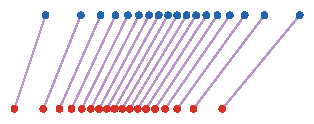
\includegraphics[width=.46\linewidth]{figures/matching-1d-convex-concave-costs--convex.pdf} &
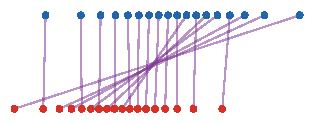
\includegraphics[width=.46\linewidth]{figures/matching-1d-convex-concave-costs--concave.pdf} \\[-.1em]
\small convex cost, $p=2$ &
\small concave cost, $p=1/2$ \\[.25em]
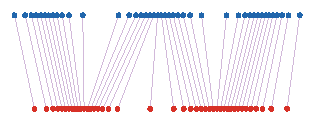
\includegraphics[width=.46\linewidth]{figures/matching-1d-convex-concave-costs--mixture-convex.pdf} &
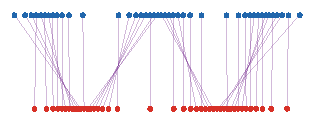
\includegraphics[width=.46\linewidth]{figures/matching-1d-convex-concave-costs--mixture-concave.pdf} \\[-.1em]
\small two-mode to three-mode, $p=2$ &
\small two-mode to three-mode, $p=1/2$
\end{tabular}
\caption{One-dimensional assignments for ordered source and target clouds with costs $c_p(x,y)=|x-y|^p$. The top row uses single-Gaussian source and target clouds; the bottom row uses a denser two-component source and three-component target. For the convex quadratic cost, equal ranks are matched and the segments do not cross. For the concave cost, the optimum creates long crossing exchanges; the ordered line remains useful, but through the alternating-chain structure of concave transport rather than through monotone rearrangement.}
\index{monotone!rearrangement}% strictindex
\index{cost!quadratic}% strictindex
\label{fig:matching-1d-convex-concave-costs}
\end{figure}

\begin{figure}[ht]
\centering
\begin{tabular}{@{}cc@{}}
\small two mixtures & \small one mode to three modes \\[-.15em]
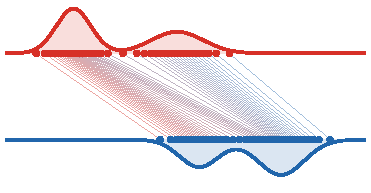
\includegraphics[width=.46\linewidth]{figures/matching-1d-quantile-assignment--quantile-assignment.pdf} &
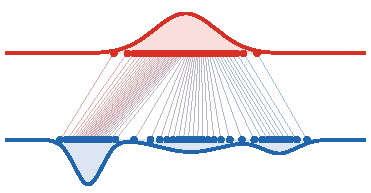
\includegraphics[width=.46\linewidth]{figures/matching-1d-quantile-assignment--central-to-three-modes.pdf}
\end{tabular}
\caption{One-dimensional optimal matching by quantile sorting. The red and blue curves are smooth laws used to generate equal-weight empirical measures; the dots are inverse-CDF samples at common quantile levels. The monotone assignment connects equal ranks, both for two Gaussian mixtures and for the transport from one central Gaussian toward a three-mode target law.}
\index{Gaussian mixture}% strictindex
\index{empirical!measure}% strictindex
\label{fig:matching-1d-quantile-assignment}
\end{figure}

%
Note that if $\phi : \RR \rightarrow \RR$ is an increasing map, one can apply this technique to costs of the form $h(|\phi(x)-\phi(y)|)$ with a change of variable.
%
A typical application is grayscale histogram equalization. The empirical cumulative distribution of the luminance values of an image is transported to a prescribed target histogram, for instance a concentrated or reference-image histogram. In one dimension, the monotone rearrangement above gives the exact transport map, so the operation is both computationally simple and geometrically faithful: it matches distributions of intensities rather than individual pixels.
\index{histogram}% strictindex
\index{transport map}% strictindex
\index{monotone!rearrangement}% strictindex

\begin{figure}[H]
\centering
\begin{tabular}{@{}cccc@{}}
\small $t=0$ & \small $t=1/3$ & \small $t=2/3$ & \small $t=1$ \\[-.15em]
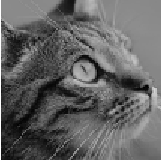
\includegraphics[width=.21\linewidth]{figures/monge-histogram-equalization--image-t000.pdf} &
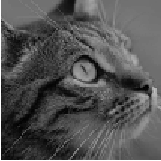
\includegraphics[width=.21\linewidth]{figures/monge-histogram-equalization--image-t033.pdf} &
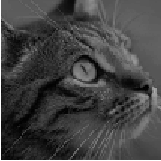
\includegraphics[width=.21\linewidth]{figures/monge-histogram-equalization--image-t067.pdf} &
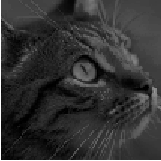
\includegraphics[width=.21\linewidth]{figures/monge-histogram-equalization--image-t100.pdf} \\[-.1em]
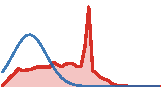
\includegraphics[width=.21\linewidth]{figures/monge-histogram-equalization--hist-t000.pdf} &
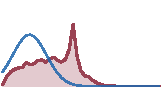
\includegraphics[width=.21\linewidth]{figures/monge-histogram-equalization--hist-t033.pdf} &

\includegraphics[width=.21\linewidth]{figures/monge-histogram-equalization--hist-t067.pdf} &

\includegraphics[width=.21\linewidth]{figures/monge-histogram-equalization--hist-t100.pdf}
\end{tabular}
\caption{Histogram equalization as one-dimensional Monge transport on pixel intensities. The map is the monotone rearrangement $T=Q_\beta\circ F_\alpha$, using the cumulative and quantile functions defined later in Definition~\ref{def-cdf-quantile}; here $\beta$ is a truncated Gaussian concentrated near dark intensities. The images are interpolated pointwise by $I_t=(1-t)I+tT(I)$, and all histograms share the same vertical scale to make the displacement of intensity mass comparable across time.}
\index{cumulative!function}% strictindex
\index{quantile!function}% strictindex
\index{monotone!rearrangement}% strictindex
\label{fig:monge-histogram-equalization}
\end{figure}

Note that if $h$ is strictly convex, then all optimal assignments are increasing, and if the points are all distinct, this increasing map is unique. If $h$ is not strictly convex, for instance $c(x,y)=|x-y|$, non-increasing optimal assignments can also exist. This happens, for example, in the book-shifting problem with overlapping uniform distributions, where the mass in the intersection can stay fixed.

\paragraph{Optimal transport on the circle.}\label{rem-circle-ot-cut}
\index{circle!transport}% strictindex

The sorting rule on the line has a periodic analogue. Identify the circle with $\mathbb S^1=\RR/\ZZ$, let
\[
	d_{\mathbb S^1}(x,y):=\min_{k\in\ZZ}|x-y+k|,
	\qquad
	c_p(x,y):=d_{\mathbb S^1}(x,y)^p,\qquad p>1.
\]
The only extra datum, compared with the line, is where one opens the circle. Once a cut has been chosen, the circle is unfolded into an interval and the one-dimensional monotone assignment can be used. In the discrete case, changing the cut is the same as applying a cyclic shift to one of the two circular orderings.
\index{cyclic!shift}% strictindex

\begin{proposition}[Discrete circle transport by a cut]\label{prop-circle-ot-cut}
\index{circle!transport}% strictindex
	Let $x_1,\ldots,x_n$ and $y_1,\ldots,y_n$ be two families of distinct points on $\mathbb S^1$, with equal weights. Let $x_{(1)},\ldots,x_{(n)}$ and $y_{(1)},\ldots,y_{(n)}$ denote any fixed cyclic orderings, with the convention $y_{(k+n)}=y_{(k)}$. For the cost $c_p$, $p>1$, an optimal assignment is one of the cyclic shifts
	\[
		x_{(k)}\longmapsto y_{(k+s)},\qquad k\in\range{n},\quad s\in\{0,\ldots,n-1\},
	\]
	and is found by minimizing
	\[
		\sum_{k=1}^n d_{\mathbb S^1}\!\left(x_{(k)},y_{(k+s)}\right)^p
	\]
	over the $n$ possible shifts. Equivalently, for an optimal shift one can choose a cut $\theta\in\mathbb S^1\setminus(\{x_i\}_i\cup\{y_j\}_j)$ so that, after lifting all points to $(\theta,\theta+1)$ and sorting them, the optimal matching is the equal-rank monotone matching on this interval.
\index{monotone!matching}% strictindex
\end{proposition}

\begin{proof}
	Call two matched pairs cyclically inverted if the circular order of their source endpoints is opposite to the circular order of their target endpoints. Among optimal assignments, choose one with the smallest number of such inversions. The elementary exchange step is the circular analogue of the line argument in Proposition~\ref{prop-matching-1d-monotone}: if two matched pairs are inverted, then cutting the circle in a gap which does not meet the four endpoints and choosing integer lifts realizes the four geodesic distances involved in the exchange as ordinary distances between two ordered source lifts and two oppositely ordered target lifts. The one-dimensional Monge inequality for the strictly convex function $r\mapsto |r|^p$ then shows that swapping the two targets cannot increase the cost, and decreases it unless the four endpoints are in a degenerate tie configuration.
\index{convex!function}% strictindex
	
	Thus an optimal assignment can be chosen with no cyclic inversion. A bijection between two finite cyclically ordered sets with no cyclic inversion is a rotation of the order, hence a cyclic shift. This shift specifies how the two cyclic orderings should be opened; after this cut, the rotation becomes an ordinary linear order and the matching is the equal-rank monotone assignment on the unfolded interval. Conversely, each cut gives one such cyclic shift, so minimizing over the finitely many shifts gives an optimal discrete circle assignment. Repeated points or ties are obtained by the same argument after an arbitrarily small perturbation and a limiting passage. This is the discrete form of the fast circle-Monge construction of~\cite{delon-circle}.
\index{circle!unfolded interval}% strictindex
\index{cyclic!shift}% strictindex
\end{proof}

\begin{alg}[Circle assignment by cutting]\label{alg:circle-cut-assignment}
\textbf{Input:} Equal-weight points $(x_i)_{i=1}^n$, $(y_j)_{j=1}^n$ on $\mathbb S^1$; cost $d_{\mathbb S^1}^p$.

\textbf{Output:} Optimal cyclic assignment.

\textbf{Let} $x_{(1)},\ldots,x_{(n)}$ and $y_{(1)},\ldots,y_{(n)}$ be the points sorted by increasing angle from a fixed origin.

\textbf{For} $s=0,\ldots,n-1$ \textbf{do}:
\begin{algblock}
\(E_s=\sum_{k=1}^n d_{\mathbb S^1}\!\left(x_{(k)},y_{(k+s)}\right)^p, \qquad y_{(k+n)}=y_{(k)}.\)
\end{algblock}
\textbf{Set} $s^\star=\min\argmin_{0\leq s<n}E_s$.

\textbf{Set} $\theta_{\rm cut}$ in an empty arc separating two consecutive matched pairs for the shift $s^\star$.

\textbf{Replace} every angle by its representative in $[\theta_{\rm cut},\theta_{\rm cut}+2\pi)$.
\textbf{Return} $x_{(k)}\mapsto y_{(k+s^\star)}$.
\end{alg}

\begin{figure}[htbp]
\centering
\begin{tabular}{cc}
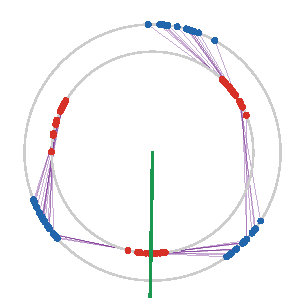
\includegraphics[width=.34\linewidth]{figures/monge-circle-cut-unfolding--circle.pdf} &
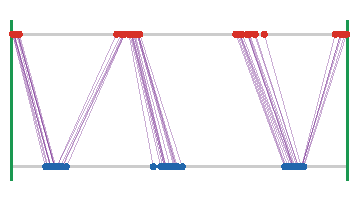
\includegraphics[width=.52\linewidth]{figures/monge-circle-cut-unfolding--unfolded.pdf} \\[-.1em]
\small circular problem &
\small unfolded interval
\index{circle!unfolded interval}% strictindex
\end{tabular}
\caption{Optimal transport on the circle by cutting and unfolding. The red and blue atoms live on two copies of the circle; the denser point clouds make the cyclic ordering visible. Purple segments show the optimal matching and the green radius marks the chosen cut. Once the circle is opened at this angle, the same matching appears as a monotone one-dimensional assignment on the interval, with the two green endpoints identified.}
\index{circle!transport}% strictindex
\label{fig:monge-circle-cut-unfolding}
\end{figure}

\begin{figure}[ht]
\centering
\begin{tabular}{ccc}
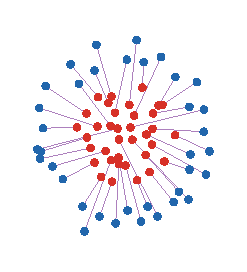
\includegraphics[width=.30\linewidth]{figures/matching-2d-cost-exponent--p1.pdf} &
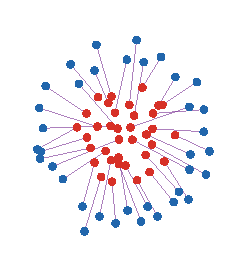
\includegraphics[width=.30\linewidth]{figures/matching-2d-cost-exponent--p2.pdf} &
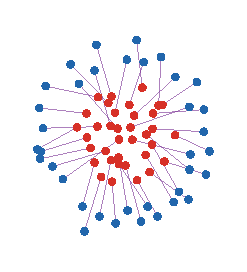
\includegraphics[width=.30\linewidth]{figures/matching-2d-cost-exponent--p6.pdf} \\[-.1em]
\small $c(x,y)=\norm{x-y}$ &
\small $c(x,y)=\norm{x-y}^2$ &
\small $c(x,y)=\norm{x-y}^6$
\end{tabular}
\caption{Optimal assignments between the same two point clouds for three powers of the Euclidean distance. The source atoms are semi-regular samples in a central disk, while the target atoms are semi-regular samples on a thin annulus; this canonical geometry is reused in later coupling and regularization figures. The feasible set is unchanged, but increasing $p$ penalizes the longest edges more strongly and changes the global organization of the permutation.}
\label{fig:matching-2d-cost-exponent}
\end{figure}

\paragraph{Rational weights.}
\index{rational weights}% strictindex

The strict assignment model is also tied to equal cardinalities and equal weights. As soon as the target resolution changes or the weights are not uniform, a permutation no longer describes the feasible transports. One instead needs a nonnegative transport matrix with prescribed row and column sums, as illustrated in Figure~\ref{fig:matching-resolution-and-weights}; this is the finite-dimensional Kantorovich relaxation developed in Chapter~\ref{sec-kantorovich}.
\index{matrix!nonnegative transport}% strictindex
\index{Kantorovich!relaxation}% strictindex

\begin{figure}[ht]
\centering
\begin{tabular}{ccc}
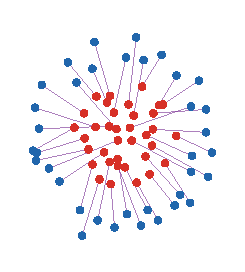
\includegraphics[width=.30\linewidth]{figures/matching-resolution-and-weights--balanced.pdf} &
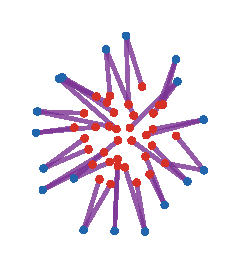
\includegraphics[width=.30\linewidth]{figures/matching-resolution-and-weights--rectangular.pdf} &
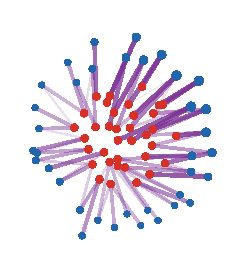
\includegraphics[width=.30\linewidth]{figures/matching-resolution-and-weights--weighted.pdf} \\[-.1em]
\small $n=m$ &
\small $m<n$ &
\small $n=m$ but $\b_j\neq 1/n$
\end{tabular}
\caption{From assignments to transport plans, using the same disk-to-annulus geometry as Figure~\ref{fig:matching-2d-cost-exponent}. In the balanced equal-weight case, each source atom is matched to one target atom. With a target cloud that has half as many atoms, or with strongly nonuniform target weights, the coupling matrix can merge or split mass; segment thickness and opacity encode its nonzero entries, and blue marker areas encode the prescribed target masses.}
\index{plan!transport}% strictindex
\label{fig:matching-resolution-and-weights}
\end{figure}

\begin{proposition}[Rational weights as duplicated uniform matching]\label{prop-rational-weights-duplicated-matching}
\index{rational weights}% strictindex
\index{matching!uniform}% strictindex
	Let
	\[
		\mu=\sum_{i=1}^n \frac{k_i}{N}\delta_{x_i},
		\qquad
		\nu=\sum_{j=1}^m \frac{\ell_j}{N}\delta_{y_j},
		\qquad
		\sum_i k_i=\sum_j\ell_j=N,
	\]
	with $k_i,\ell_j\in\NN$. The discrete Kantorovich problem between $(\mu,\nu)$ is equivalent to the uniform assignment problem obtained by replacing each $x_i$ by $k_i$ identical copies and each $y_j$ by $\ell_j$ identical copies. More precisely, after multiplying transport masses by $N$, optimal couplings correspond to optimal integer count matrices $(n_{ij})$ with row sums $k_i$ and column sums $\ell_j$, and these count matrices are exactly the collapsed form of assignments between the duplicated clouds.
\index{Kantorovich!problem}% strictindex
\index{optimal coupling}% strictindex
\index{assignment problem}% strictindex
\end{proposition}
\begin{proof}
	Any assignment between the duplicated source and target clouds defines integers $n_{ij}$ counting how many copied particles of type $x_i$ are matched to copied particles of type $y_j$. These counts satisfy $\sum_j n_{ij}=k_i$ and $\sum_i n_{ij}=\ell_j$, and the associated coupling $P_{ij}=n_{ij}/N$ has marginals $k_i/N$ and $\ell_j/N$. The assignment cost is
\index{cost!assignment}% strictindex
	\[
		\frac1N\sum_{i,j} n_{ij}c(x_i,y_j)
		=
		\sum_{i,j}P_{ij}c(x_i,y_j).
	\]
	Conversely, any nonnegative integer count matrix with those row and column sums can be realized by matching the corresponding duplicated particles. Finally, the transportation constraint matrix is totally unimodular, so the linear problem with integer supplies and demands has an optimal integer count matrix. Thus the optimum of the rational-weight Kantorovich problem is the same as the optimum of the duplicated uniform assignment problem.
\index{assignment problem}% strictindex
\end{proof}

\begin{figure}[ht]
\centering
\begin{tabular}{ccc}
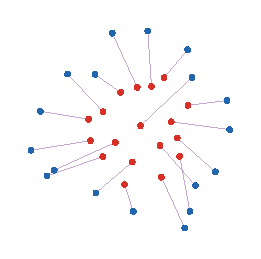
\includegraphics[width=.30\linewidth]{figures/matching-rational-duplication--uniform.pdf} &
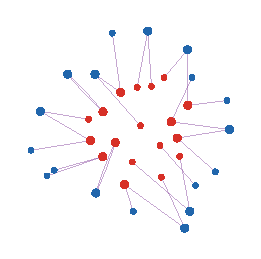
\includegraphics[width=.30\linewidth]{figures/matching-rational-duplication--binary.pdf} &
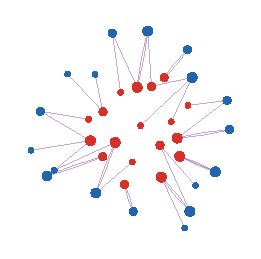
\includegraphics[width=.30\linewidth]{figures/matching-rational-duplication--ternary.pdf} \\[-.1em]
\small $k_i=\ell_j=1$ &
\small $k_i,\ell_j\in\{1,2\}$ &
\small $k_i,\ell_j\in\{1,2,3\}$
\end{tabular}
\caption{Rational weights as duplicated uniform matchings, using the same disk-to-annulus geometry as Figure~\ref{fig:matching-resolution-and-weights} with fewer displayed atoms. The red and blue locations are kept fixed, while disk areas encode the integer multiplicities $k_i$ and $\ell_j$. Solving the assignment problem after duplicating particles produces several collapsed segments attached to high-multiplicity atoms; this is the integer count matrix of Proposition~\ref{prop-rational-weights-duplicated-matching}.}
\index{integer multiplicity}% strictindex
\index{assignment problem}% strictindex
\index{rational weights}% strictindex
\index{matching!uniform}% strictindex
\label{fig:matching-rational-duplication}
\end{figure}

\paragraph{2D case.}

This efficient strategy to compute the OT in 1-D does not extend to higher dimensions. In 2-D, as already noted by Monge, one has the following property.

\begin{proposition}[Non-crossing optimal matchings]
\index{matching!non-crossing}% strictindex
	In dimension 2, for $c(x,y) = \norm{x-y}$, if $\sigma$ is an optimal assignment, then segments $[x_i,y_{\sigma(i)}]$ cannot cross.
\end{proposition}

\begin{proof}
	If two segments $[x_i,y_{\sigma(i)}]$ and $[x_j,y_{\sigma(j)}]$ cross at an interior point $z$, then the triangle inequality gives
\index{triangle inequality}% strictindex
	\[
		\norm{x_i-y_{\sigma(j)}}+\norm{x_j-y_{\sigma(i)}}
		<
		\norm{x_i-y_{\sigma(i)}}+\norm{x_j-y_{\sigma(j)}}.
	\]
	The assignment obtained by swapping $(\sigma(i),\sigma(j))$ therefore has a strictly smaller cost, which contradicts optimality.
\end{proof}

This property alone is, however, not enough to lead to an efficient algorithm. Non-crossing is only a necessary local test, not a compact certificate of optimality. For instance, if $n$ sources and $n$ targets are placed alternately on the boundary of a convex polygon, the number of non-crossing perfect matchings is the Catalan number
\index{matching!perfect}% strictindex
\index{Catalan number}% strictindex
\[
	C_n=\frac{1}{n+1}\binom{2n}{n}\sim \frac{4^n}{\sqrt{\pi}n^{3/2}}.
\]

\begin{rem}[Catalan count of alternating non-crossing matchings]
\index{matching!non-crossing}% strictindex
	The count follows from the standard Catalan recurrence. Fix one red vertex $r$. In a non-crossing perfect matching, if $r$ is matched to a blue vertex $b$, the chord $[r,b]$ splits the polygon into two smaller polygons. Since the boundary colors alternate, each side contains the same number of red and blue vertices. If one side contains $k$ red and $k$ blue vertices, the other contains $n-1-k$ red and $n-1-k$ blue vertices. Non-crossing matchings on the two sides are independent, because no segment can cross the chord $[r,b]$. Thus, denoting by $M_n$ the number of such matchings, one has
\index{matching!perfect}% strictindex
	\[
		M_0=1,
		\qquad
		M_n=\sum_{k=0}^{n-1} M_k M_{n-1-k}.
	\]
	This recurrence characterizes the Catalan numbers, hence $M_n=C_n$.
\index{Catalan number}% strictindex
\end{rem}

Thus even after forbidding crossings, an exhaustive search remains exponential. The two-segment swap in the proof above is nevertheless useful: it explains why a crossing matching cannot be optimal, but it does not select among the exponentially many planar matchings that survive this local test.


%%%%%%%%%%%%%%%%%%%%%%%%%%%%%%%%%%%%%%%%%%%%%%%%%%%%%%%%%%%%%%%%%%%%%%%%%%%
\section{Matching Algorithms}
\index{matching!algorithm}% strictindex

This section briefly locates matching within classical combinatorial optimization. Its main point is that efficient algorithms exist, but their cleanest analysis is obtained only after introducing the linear-programming viewpoint.

Efficient algorithms exist to solve the optimal matching problem. The most well-known are the Hungarian method and auction algorithms~\cite{Kuhn1955,bertsekas1981new,bertsekas1992auction}. Auction algorithms use prices on the target points: each source bids for the target with largest reduced profit, the target price is increased, and the process terminates when the $\epsilon$-complementary slackness conditions are satisfied. For integer costs, choosing $\epsilon<1/n$ gives an exact optimum after a finite number of bids~\cite{bertsekas1992auction}. Section~\ref{sec-auction-dual-ascent} revisits this algorithm after Kantorovich duality and explains why it is a dual price method, parallel in spirit to Sinkhorn scaling.
\index{Sinkhorn!scaling}% strictindex
\index{Hungarian primal-dual method}% strictindex
\index{optimality!complementary slackness}% strictindex
\index{Kantorovich!duality}% strictindex
\index{auction algorithm}% strictindex
\index{assignment problem}% strictindex

\paragraph{Hungarian primal-dual method.}
\index{Hungarian primal-dual method}% strictindex

The Hungarian method is best understood as a certificate-building algorithm for the assignment linear program. It maintains a partial matching $M$ and dual prices $(u_i,v_j)$ satisfying
\[
	u_i+v_j\leq C_{i,j}\qquad\forall i,j.
\]
The equality graph $E(u,v)=\{(i,j):u_i+v_j=C_{i,j}\}$ contains the edges whose reduced cost is zero. The algorithm only augments $M$ along alternating paths made of equality edges. Starting from an unmatched source, it grows an alternating tree with source set $S$ and target set $T$. If the tree reaches an unmatched target, the matching is augmented along the path. If no such edge exists, the dual variables are shifted by the smallest slack
\index{alternating!tree}% strictindex
\index{graph!equality}% strictindex
\index{cost!reduced}% strictindex
\[
	\delta=\min_{i\in S,\ j\notin T}\bigl(C_{i,j}-u_i-v_j\bigr),
	\qquad
	u_i\leftarrow u_i+\delta\ (i\in S),\qquad
	v_j\leftarrow v_j-\delta\ (j\in T).
\]
This update preserves all inequalities $u_i+v_j\leq C_{i,j}$, keeps the current alternating tree tight, and creates at least one new equality edge leaving $S$. Maintaining these slacks incrementally gives the standard $O(n^3)$ implementation for an $n\times n$ assignment problem.
\index{assignment problem}% strictindex
\index{alternating!tree}% strictindex
Algorithm~\ref{alg:hungarian-primal-dual} summarizes the primal-dual loop. Figure~\ref{fig:matching-hungarian-progression} displays actual iterates by showing only the evolving partial assignment: unmatched rows are shown as flat rows to keep a fixed matrix format, and matched rows are shown as one-hot rows.
\index{Hungarian primal-dual method}% strictindex

\begin{alg}[Hungarian primal-dual augmentation]\label{alg:hungarian-primal-dual}
\textbf{Input:} Square cost matrix $C\in\RR^{n\times n}$.

\textbf{Output:} Minimum-cost perfect matching $M$.

\textbf{Initialize:} Set $u_i=\min_j C_{ij}$ and $v_j=0$.

\textbf{Set} $M=\emptyset$.

\textbf{While} $M$ is not perfect \textbf{do}:
\begin{algblock}

\textbf{Build} equality graph:
\(E(u,v)=\{(i,j):u_i+v_j=C_{i,j}\}.\)

\textbf{Set} root $i_0=\min\{i:\ i\text{ is unmatched in }M\}$.

\textbf{Set} reached sets $S=\{i_0\}$ and $T=\emptyset$; clear parent pointers.

\textbf{While} $T$ contains no unmatched target \textbf{do}:
\begin{algblock}

\textbf{If} $N_E(S)\setminus T=\emptyset$ \textbf{then}:
\begin{algblock}

\textbf{Compute} $\delta=\min_{i\in S,\ j\notin T}\bigl(C_{i,j}-u_i-v_j\bigr)$.

\textbf{Update} $u_i\leftarrow u_i+\delta$ for $i\in S$ and $v_j\leftarrow v_j-\delta$ for $j\in T$.

\textbf{Refresh} equality graph $E(u,v)$.

\end{algblock}
\textbf{Set} $J=N_E(S)\setminus T$.

\textbf{For} each $j\in J$ in increasing order \textbf{do}:
\begin{algblock}

\textbf{Add} $j$ to $T$ and set parent row $p(j)=\min\{i\in S:(i,j)\in E(u,v)\}$.

\textbf{If} $j$ is matched to $i'$ in $M$ \textbf{then set} \(S\leftarrow S\cup\{i'\}\) and \(q(i')=j\).

\end{algblock}
\end{algblock}
\textbf{Set} $j_0=\min\{j\in T:\ j\text{ is unmatched in }M\}$.

\textbf{Set} $j=j_0$.

\textbf{While} $j$ is defined \textbf{do}:
\begin{algblock}

\textbf{Set} $i=p(j)$.

\textbf{Set} $M\leftarrow M\cup\{(i,j)\}$.

\textbf{Set} $j_{\rm old}=q(i)$.

\textbf{If} $j_{\rm old}$ is defined \textbf{then set} \(M\leftarrow M\setminus\{(i,j_{\rm old})\}\).
\textbf{Set} $j=j_{\rm old}$.
\end{algblock}
\end{algblock}
\algreturnskip
\textbf{Return} $M$.
\end{alg}

\begin{figure}[ht]
\centering
\setlength{\tabcolsep}{2pt}
\begin{tabular}{ccccc}
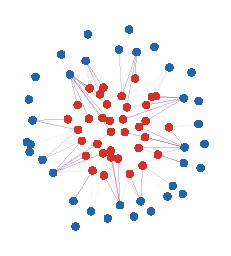
\includegraphics[width=.18\linewidth]{figures/matching-hungarian-progression--stage-0.pdf} &
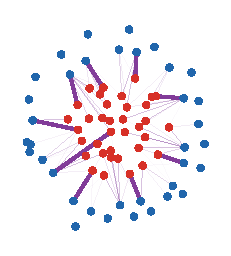
\includegraphics[width=.18\linewidth]{figures/matching-hungarian-progression--stage-1.pdf} &
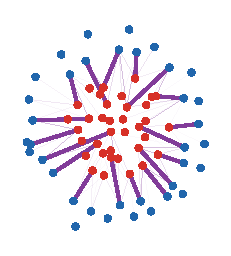
\includegraphics[width=.18\linewidth]{figures/matching-hungarian-progression--stage-2.pdf} &
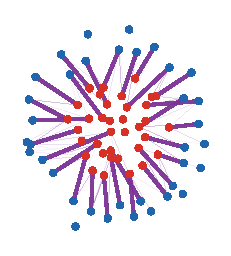
\includegraphics[width=.18\linewidth]{figures/matching-hungarian-progression--stage-3.pdf} &
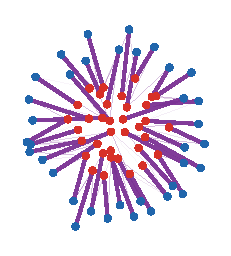
\includegraphics[width=.18\linewidth]{figures/matching-hungarian-progression--stage-4.pdf} \\[-.1em]
\small initial &
\small 2 aug. &
\small 4 aug. &
\small 6 aug. &
\small final
\end{tabular}
\caption{Matrix view of actual Hungarian primal-dual iterates on a diagonally dominant ordered one-dimensional squared-distance assignment. Each panel records the current partial assignment state: unassigned rows are kept flat, while assigned rows are one-hot. The snapshots are taken at initialization and after two, four, six and eight augmentations; for this pedagogical instance the partial assignments grow along the diagonal, and the final matrix is the identity assignment certified by complementary slackness.}
\index{optimality!complementary slackness}% strictindex
\label{fig:matching-hungarian-progression}
\end{figure}

\begin{prop}[Correctness and complexity of the Hungarian primal-dual method]\label{prop-hungarian-correct}
\index{Hungarian primal-dual method}% strictindex
	Assume the Hungarian method terminates with a perfect matching $\sigma$ contained in the equality graph
\index{matching!perfect}% strictindex
\index{graph!equality}% strictindex
	\[
		E(u,v)=\enscond{(i,j)}{u_i+v_j=C_{i,j}},
	\]
	where $(u,v)$ is dual feasible, i.e. $u_i+v_j\leq C_{i,j}$ for all $(i,j)$. Then $\sigma$ is an optimal assignment. Moreover, the usual Hungarian updates terminate after finitely many augmentations.
\index{Hungarian primal-dual method}% strictindex
	With maintained slacks, the method uses $O(n^3)$ arithmetic operations.
\end{prop}

\begin{proof}
	For any permutation $\tau$, dual feasibility gives
	\[
		\sum_i C_{i,\tau(i)} \geq \sum_i (u_i+v_{\tau(i)})
		= \sum_i u_i+\sum_j v_j.
	\]
	This is the weak duality lower bound. If $\sigma$ is contained in the equality graph, then
\index{duality!weak}% strictindex
\index{graph!equality}% strictindex
	\[
		\sum_i C_{i,\sigma(i)}
		= \sum_i u_i+\sum_j v_j,
	\]
	so the primal cost of $\sigma$ reaches the dual lower bound and is optimal.

	It remains to justify finite termination and the complexity bound. At each successful augmentation, the matching cardinality increases by one, so there are at most $n$ augmentations. During one augmentation phase, the algorithm grows an alternating tree in the equality graph. If no augmenting path is available, the dual update uses the smallest slack of an edge leaving the current tree. For edges inside the tree, adding $\delta$ to source labels and subtracting $\delta$ from target labels preserves tightness; for edges from $S$ to $T^c$, the definition of $\delta$ preserves feasibility and makes at least one new edge tight; all other inequalities are unchanged or become looser. Thus the reachable sets strictly grow between two failed augmentation attempts, and they can grow at most $n$ times within one phase. If the current slacks $\min_{i\in S}(C_{i,j}-u_i-v_j)$ are updated when a source enters $S$, each tree expansion costs $O(n)$. A phase therefore costs $O(n^2)$, and the $n$ phases give $O(n^3)$ operations. Hence the method reaches a perfect optimal matching.
\index{tightness}% strictindex
\index{alternating!tree}% strictindex
\index{graph!augmenting path}% strictindex
\index{graph!equality}% strictindex
\end{proof}
